\documentclass[1p]{elsarticle_modified}
%\bibliographystyle{elsarticle-num}

%\usepackage[colorlinks]{hyperref}
%\usepackage{abbrmath_seonhwa} %\Abb, \Ascr, \Acal ,\Abf, \Afrak
\usepackage{amsfonts}
\usepackage{amssymb}
\usepackage{amsmath}
\usepackage{amsthm}
\usepackage{scalefnt}
\usepackage{amsbsy}
\usepackage{kotex}
\usepackage{caption}
\usepackage{subfig}
\usepackage{color}
\usepackage{graphicx}
\usepackage{xcolor} %% white, black, red, green, blue, cyan, magenta, yellow
\usepackage{float}
\usepackage{setspace}
\usepackage{hyperref}

\usepackage{tikz}
\usetikzlibrary{arrows}

\usepackage{multirow}
\usepackage{array} % fixed length table
\usepackage{hhline}

%%%%%%%%%%%%%%%%%%%%%
\makeatletter
\renewcommand*\env@matrix[1][\arraystretch]{%
	\edef\arraystretch{#1}%
	\hskip -\arraycolsep
	\let\@ifnextchar\new@ifnextchar
	\array{*\c@MaxMatrixCols c}}
\makeatother %https://tex.stackexchange.com/questions/14071/how-can-i-increase-the-line-spacing-in-a-matrix
%%%%%%%%%%%%%%%

\usepackage[normalem]{ulem}

\newcommand{\msout}[1]{\ifmmode\text{\sout{\ensuremath{#1}}}\else\sout{#1}\fi}
%SOURCE: \msout is \stkout macro in https://tex.stackexchange.com/questions/20609/strikeout-in-math-mode

\newcommand{\cancel}[1]{
	\ifmmode
	{\color{red}\msout{#1}}
	\else
	{\color{red}\sout{#1}}
	\fi
}

\newcommand{\add}[1]{
	{\color{blue}\uwave{#1}}
}

\newcommand{\replace}[2]{
	\ifmmode
	{\color{red}\msout{#1}}{\color{blue}\uwave{#2}}
	\else
	{\color{red}\sout{#1}}{\color{blue}\uwave{#2}}
	\fi
}

\newcommand{\Sol}{\mathcal{S}} %segment
\newcommand{\D}{D} %diagram
\newcommand{\A}{\mathcal{A}} %arc


%%%%%%%%%%%%%%%%%%%%%%%%%%%%%5 test

\def\sl{\operatorname{\textup{SL}}(2,\Cbb)}
\def\psl{\operatorname{\textup{PSL}}(2,\Cbb)}
\def\quan{\mkern 1mu \triangleright \mkern 1mu}

\theoremstyle{definition}
\newtheorem{thm}{Theorem}[section]
\newtheorem{prop}[thm]{Proposition}
\newtheorem{lem}[thm]{Lemma}
\newtheorem{ques}[thm]{Question}
\newtheorem{cor}[thm]{Corollary}
\newtheorem{defn}[thm]{Definition}
\newtheorem{exam}[thm]{Example}
\newtheorem{rmk}[thm]{Remark}
\newtheorem{alg}[thm]{Algorithm}

\newcommand{\I}{\sqrt{-1}}
\begin{document}

%\begin{frontmatter}
%
%\title{Boundary parabolic representations of knots up to 8 crossings}
%
%%% Group authors per affiliation:
%\author{Yunhi Cho} 
%\address{Department of Mathematics, University of Seoul, Seoul, Korea}
%\ead{yhcho@uos.ac.kr}
%
%
%\author{Seonhwa Kim} %\fnref{s_kim}}
%\address{Center for Geometry and Physics, Institute for Basic Science, Pohang, 37673, Korea}
%\ead{ryeona17@ibs.re.kr}
%
%\author{Hyuk Kim}
%\address{Department of Mathematical Sciences, Seoul National University, Seoul 08826, Korea}
%\ead{hyukkim@snu.ac.kr}
%
%\author{Seokbeom Yoon}
%\address{Department of Mathematical Sciences, Seoul National University, Seoul, 08826,  Korea}
%\ead{sbyoon15@snu.ac.kr}
%
%\begin{abstract}
%We find all boundary parabolic representation of knots up to 8 crossings.
%
%\end{abstract}
%\begin{keyword}
%    \MSC[2010] 57M25 
%\end{keyword}
%
%\end{frontmatter}

%\linenumbers
%\tableofcontents
%
\newcommand\colored[1]{\textcolor{white}{\rule[-0.35ex]{0.8em}{1.4ex}}\kern-0.8em\color{red} #1}%
%\newcommand\colored[1]{\textcolor{white}{ #1}\kern-2.17ex	\textcolor{white}{ #1}\kern-1.81ex	\textcolor{white}{ #1}\kern-2.15ex\color{red}#1	}

{\Large $\underline{12n_{0020}~(K12n_{0020})}$}

\setlength{\tabcolsep}{10pt}
\renewcommand{\arraystretch}{1.6}
\vspace{1cm}\begin{tabular}{m{100pt}>{\centering\arraybackslash}m{274pt}}
\multirow{5}{120pt}{
	\centering
	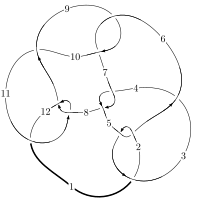
\includegraphics[width=112pt]{../../../GIT/diagram.site/Diagrams/png/2109_12n_0020.png}\\
\ \ \ A knot diagram\footnotemark}&
\allowdisplaybreaks
\textbf{Linearized knot diagam} \\
\cline{2-2}
 &
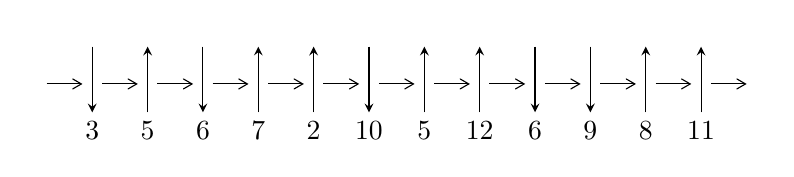
\begin{tikzpicture}[x=20pt, y=17pt]
	% nodes
	\node (C0) at (0, 0) {};
	\node (C1) at (1, 0) {};
	\node (C1U) at (1, +1) {};
	\node (C1D) at (1, -1) {3};

	\node (C2) at (2, 0) {};
	\node (C2U) at (2, +1) {};
	\node (C2D) at (2, -1) {5};

	\node (C3) at (3, 0) {};
	\node (C3U) at (3, +1) {};
	\node (C3D) at (3, -1) {6};

	\node (C4) at (4, 0) {};
	\node (C4U) at (4, +1) {};
	\node (C4D) at (4, -1) {7};

	\node (C5) at (5, 0) {};
	\node (C5U) at (5, +1) {};
	\node (C5D) at (5, -1) {2};

	\node (C6) at (6, 0) {};
	\node (C6U) at (6, +1) {};
	\node (C6D) at (6, -1) {10};

	\node (C7) at (7, 0) {};
	\node (C7U) at (7, +1) {};
	\node (C7D) at (7, -1) {5};

	\node (C8) at (8, 0) {};
	\node (C8U) at (8, +1) {};
	\node (C8D) at (8, -1) {12};

	\node (C9) at (9, 0) {};
	\node (C9U) at (9, +1) {};
	\node (C9D) at (9, -1) {6};

	\node (C10) at (10, 0) {};
	\node (C10U) at (10, +1) {};
	\node (C10D) at (10, -1) {9};

	\node (C11) at (11, 0) {};
	\node (C11U) at (11, +1) {};
	\node (C11D) at (11, -1) {8};

	\node (C12) at (12, 0) {};
	\node (C12U) at (12, +1) {};
	\node (C12D) at (12, -1) {11};
	\node (C13) at (13, 0) {};

	% arrows
	\draw[->,>={angle 60}]
	(C0) edge (C1) (C1) edge (C2) (C2) edge (C3) (C3) edge (C4) (C4) edge (C5) (C5) edge (C6) (C6) edge (C7) (C7) edge (C8) (C8) edge (C9) (C9) edge (C10) (C10) edge (C11) (C11) edge (C12) (C12) edge (C13) ;	\draw[->,>=stealth]
	(C1U) edge (C1D) (C2D) edge (C2U) (C3U) edge (C3D) (C4D) edge (C4U) (C5D) edge (C5U) (C6U) edge (C6D) (C7D) edge (C7U) (C8D) edge (C8U) (C9U) edge (C9D) (C10U) edge (C10D) (C11D) edge (C11U) (C12D) edge (C12U) ;
	\end{tikzpicture} \\
\hhline{~~} \\& 
\textbf{Solving Sequence} \\ \cline{2-2} 
 &
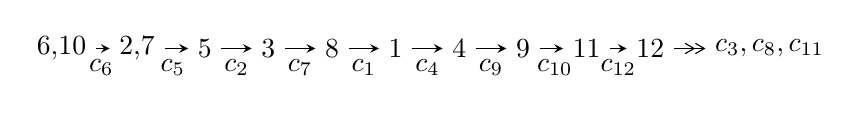
\begin{tikzpicture}[x=23pt, y=7pt]
	% node
	\node (A0) at (-1/8, 0) {6,10};
	\node (A1) at (17/16, 0) {2,7};
	\node (A2) at (17/8, 0) {5};
	\node (A3) at (25/8, 0) {3};
	\node (A4) at (33/8, 0) {8};
	\node (A5) at (41/8, 0) {1};
	\node (A6) at (49/8, 0) {4};
	\node (A7) at (57/8, 0) {9};
	\node (A8) at (65/8, 0) {11};
	\node (A9) at (73/8, 0) {12};
	\node (C1) at (1/2, -1) {$c_{6}$};
	\node (C2) at (13/8, -1) {$c_{5}$};
	\node (C3) at (21/8, -1) {$c_{2}$};
	\node (C4) at (29/8, -1) {$c_{7}$};
	\node (C5) at (37/8, -1) {$c_{1}$};
	\node (C6) at (45/8, -1) {$c_{4}$};
	\node (C7) at (53/8, -1) {$c_{9}$};
	\node (C8) at (61/8, -1) {$c_{10}$};
	\node (C9) at (69/8, -1) {$c_{12}$};
	\node (A10) at (11, 0) {$c_{3},c_{8},c_{11}$};

	% edge
	\draw[->,>=stealth]	
	(A0) edge (A1) (A1) edge (A2) (A2) edge (A3) (A3) edge (A4) (A4) edge (A5) (A5) edge (A6) (A6) edge (A7) (A7) edge (A8) (A8) edge (A9) ;
	\draw[->>,>={angle 60}]	
	(A9) edge (A10);
\end{tikzpicture} \\ 

\end{tabular} \\

\footnotetext{
The image of knot diagram is generated by the software ``\textbf{Draw programme}" developed by Andrew Bartholomew(\url{http://www.layer8.co.uk/maths/draw/index.htm\#Running-draw}), where we modified some parts for our purpose(\url{https://github.com/CATsTAILs/LinksPainter}).
}\phantom \\ \newline 
\centering \textbf{Ideals for irreducible components\footnotemark of $X_{\text{par}}$} 
 
\begin{align*}
I^u_{1}&=\langle 
6.15417\times10^{24} u^{34}+4.90608\times10^{25} u^{33}+\cdots+1.32838\times10^{26} b-6.91943\times10^{25},\\
\phantom{I^u_{1}}&\phantom{= \langle  }1.02387\times10^{26} u^{34}+2.68565\times10^{26} u^{33}+\cdots+1.32838\times10^{26} a-3.02927\times10^{26},\;u^{35}+3 u^{34}+\cdots-2 u-1\rangle \\
I^u_{2}&=\langle 
4 u^5 a+5 u^4 a+4 u^5-7 u^3 a+5 u^4-14 u^2 a-7 u^3+5 a u-14 u^2+17 b+a+5 u+1,\\
\phantom{I^u_{2}}&\phantom{= \langle  }- u^5 a+2 u^3 a-2 u^4+u^2 a- u^3+a^2-2 a u+2 u^2+2 u,\;u^6+u^5- u^4-2 u^3+u+1\rangle \\
\\
\end{align*}
\raggedright * 2 irreducible components of $\dim_{\mathbb{C}}=0$, with total 47 representations.\\
\footnotetext{All coefficients of polynomials are rational numbers. But the coefficients are sometimes approximated in decimal forms when there is not enough margin.}
\newpage
\renewcommand{\arraystretch}{1}
\centering \section*{I. $I^u_{1}= \langle 6.15\times10^{24} u^{34}+4.91\times10^{25} u^{33}+\cdots+1.33\times10^{26} b-6.92\times10^{25},\;1.02\times10^{26} u^{34}+2.69\times10^{26} u^{33}+\cdots+1.33\times10^{26} a-3.03\times10^{26},\;u^{35}+3 u^{34}+\cdots-2 u-1 \rangle$}
\flushleft \textbf{(i) Arc colorings}\\
\begin{tabular}{m{7pt} m{180pt} m{7pt} m{180pt} }
\flushright $a_{6}=$&$\begin{pmatrix}1\\0\end{pmatrix}$ \\
\flushright $a_{10}=$&$\begin{pmatrix}0\\u\end{pmatrix}$ \\
\flushright $a_{2}=$&$\begin{pmatrix}-0.770764 u^{34}-2.02174 u^{33}+\cdots-4.41998 u+2.28042\\-0.0463282 u^{34}-0.369327 u^{33}+\cdots+0.317345 u+0.520890\end{pmatrix}$ \\
\flushright $a_{7}=$&$\begin{pmatrix}1\\u^2\end{pmatrix}$ \\
\flushright $a_{5}=$&$\begin{pmatrix}1.26890 u^{34}+2.84616 u^{33}+\cdots-4.14141 u+0.782118\\-0.0631189 u^{34}-0.437170 u^{33}+\cdots+0.413577 u-0.482385\end{pmatrix}$ \\
\flushright $a_{3}=$&$\begin{pmatrix}1.55412 u^{34}+3.44078 u^{33}+\cdots-4.40019 u-0.146776\\-0.0448946 u^{34}-0.427369 u^{33}+\cdots+0.806983 u-0.450739\end{pmatrix}$ \\
\flushright $a_{8}=$&$\begin{pmatrix}0.690375 u^{34}+2.08177 u^{33}+\cdots-1.15296 u-2.07734\\0.00686562 u^{34}+0.115030 u^{33}+\cdots-0.332383 u-0.172479\end{pmatrix}$ \\
\flushright $a_{1}=$&$\begin{pmatrix}0.700744 u^{34}+1.98651 u^{33}+\cdots-0.108902 u-1.89421\\0.0103696 u^{34}-0.0952592 u^{33}+\cdots+1.04406 u+0.183128\end{pmatrix}$ \\
\flushright $a_{4}=$&$\begin{pmatrix}1.59901 u^{34}+3.86815 u^{33}+\cdots-5.20717 u+0.303962\\-0.0448946 u^{34}-0.427369 u^{33}+\cdots+0.806983 u-0.450739\end{pmatrix}$ \\
\flushright $a_{9}=$&$\begin{pmatrix}u\\u\end{pmatrix}$ \\
\flushright $a_{11}=$&$\begin{pmatrix}- u^3\\- u^3+u\end{pmatrix}$ \\
\flushright $a_{12}=$&$\begin{pmatrix}0.743963 u^{34}+2.07828 u^{33}+\cdots-0.147237 u-1.89598\\0.0883859 u^{34}+0.102670 u^{33}+\cdots+1.52166 u+0.0975759\end{pmatrix}$\\&\end{tabular}
\flushleft \textbf{(ii) Obstruction class $= -1$}\\~\\
\flushleft \textbf{(iii) Cusp Shapes $= \frac{138501011022536071388354471}{22139732193931699544465805} u^{34}+\frac{368226358523013848196048853}{22139732193931699544465805} u^{33}+\cdots-\frac{423513858408885950087940661}{44279464387863399088931610} u-\frac{130309672706343830288860133}{14759821462621133029643870}$}\\~\\
\newpage\renewcommand{\arraystretch}{1}
\flushleft \textbf{(iv) u-Polynomials at the component}\newline \\
\begin{tabular}{m{50pt}|m{274pt}}
Crossings & \hspace{64pt}u-Polynomials at each crossing \\
\hline $$\begin{aligned}c_{1}\end{aligned}$$&$\begin{aligned}
&u^{35}+5 u^{34}+\cdots+6 u-1
\end{aligned}$\\
\hline $$\begin{aligned}c_{2},c_{5}\end{aligned}$$&$\begin{aligned}
&u^{35}+7 u^{34}+\cdots-6 u-1
\end{aligned}$\\
\hline $$\begin{aligned}c_{3}\end{aligned}$$&$\begin{aligned}
&u^{35}-7 u^{34}+\cdots-25346 u-337
\end{aligned}$\\
\hline $$\begin{aligned}c_{4},c_{7}\end{aligned}$$&$\begin{aligned}
&u^{35}+3 u^{34}+\cdots+16384 u+4096
\end{aligned}$\\
\hline $$\begin{aligned}c_{6},c_{9}\end{aligned}$$&$\begin{aligned}
&u^{35}+3 u^{34}+\cdots-2 u-1
\end{aligned}$\\
\hline $$\begin{aligned}c_{8},c_{11}\end{aligned}$$&$\begin{aligned}
&u^{35}+3 u^{34}+\cdots+2 u-1
\end{aligned}$\\
\hline $$\begin{aligned}c_{10}\end{aligned}$$&$\begin{aligned}
&u^{35}+3 u^{34}+\cdots-2 u+1
\end{aligned}$\\
\hline $$\begin{aligned}c_{12}\end{aligned}$$&$\begin{aligned}
&u^{35}-23 u^{34}+\cdots-2 u-1
\end{aligned}$\\
\hline
\end{tabular}\\~\\
\newpage\renewcommand{\arraystretch}{1}
\flushleft \textbf{(v) Riley Polynomials at the component}\newline \\
\begin{tabular}{m{50pt}|m{274pt}}
Crossings & \hspace{64pt}Riley Polynomials at each crossing \\
\hline $$\begin{aligned}c_{1}\end{aligned}$$&$\begin{aligned}
&y^{35}+57 y^{34}+\cdots+6 y-1
\end{aligned}$\\
\hline $$\begin{aligned}c_{2},c_{5}\end{aligned}$$&$\begin{aligned}
&y^{35}+5 y^{34}+\cdots+6 y-1
\end{aligned}$\\
\hline $$\begin{aligned}c_{3}\end{aligned}$$&$\begin{aligned}
&y^{35}+109 y^{34}+\cdots+279652022 y-113569
\end{aligned}$\\
\hline $$\begin{aligned}c_{4},c_{7}\end{aligned}$$&$\begin{aligned}
&y^{35}-65 y^{34}+\cdots-83886080 y-16777216
\end{aligned}$\\
\hline $$\begin{aligned}c_{6},c_{9}\end{aligned}$$&$\begin{aligned}
&y^{35}-3 y^{34}+\cdots-2 y-1
\end{aligned}$\\
\hline $$\begin{aligned}c_{8},c_{11}\end{aligned}$$&$\begin{aligned}
&y^{35}-23 y^{34}+\cdots-2 y-1
\end{aligned}$\\
\hline $$\begin{aligned}c_{10}\end{aligned}$$&$\begin{aligned}
&y^{35}+61 y^{34}+\cdots+6 y-1
\end{aligned}$\\
\hline $$\begin{aligned}c_{12}\end{aligned}$$&$\begin{aligned}
&y^{35}-19 y^{34}+\cdots+182 y-1
\end{aligned}$\\
\hline
\end{tabular}\\~\\
\newpage\flushleft \textbf{(vi) Complex Volumes and Cusp Shapes}
$$\begin{array}{c|c|c}  
\text{Solutions to }I^u_{1}& \I (\text{vol} + \sqrt{-1}CS) & \text{Cusp shape}\\
 \hline 
\begin{aligned}
u &= -0.991966 + 0.091776 I \\
a &= \phantom{-}0.72692 + 1.45829 I \\
b &= -0.068558 + 0.738981 I\end{aligned}
 & -2.80047 + 0.03393 I & -4.96122 - 0.73381 I \\ \hline\begin{aligned}
u &= -0.991966 - 0.091776 I \\
a &= \phantom{-}0.72692 - 1.45829 I \\
b &= -0.068558 - 0.738981 I\end{aligned}
 & -2.80047 - 0.03393 I & -4.96122 + 0.73381 I \\ \hline\begin{aligned}
u &= \phantom{-}0.909482 + 0.380777 I \\
a &= \phantom{-}0.29144 - 1.73248 I \\
b &= \phantom{-}0.014187 - 1.000160 I\end{aligned}
 & -1.72254 - 4.24984 I & -2.18876 + 7.04122 I \\ \hline\begin{aligned}
u &= \phantom{-}0.909482 - 0.380777 I \\
a &= \phantom{-}0.29144 + 1.73248 I \\
b &= \phantom{-}0.014187 + 1.000160 I\end{aligned}
 & -1.72254 + 4.24984 I & -2.18876 - 7.04122 I \\ \hline\begin{aligned}
u &= \phantom{-}0.576907 + 0.754246 I \\
a &= \phantom{-}0.591225 + 0.311198 I \\
b &= -0.377861 - 0.131381 I\end{aligned}
 & \phantom{-}2.25585 + 1.15466 I & \phantom{-}4.96533 - 0.29519 I \\ \hline\begin{aligned}
u &= \phantom{-}0.576907 - 0.754246 I \\
a &= \phantom{-}0.591225 - 0.311198 I \\
b &= -0.377861 + 0.131381 I\end{aligned}
 & \phantom{-}2.25585 - 1.15466 I & \phantom{-}4.96533 + 0.29519 I \\ \hline\begin{aligned}
u &= -1.010040 + 0.446446 I \\
a &= \phantom{-}0.650598 - 0.883449 I \\
b &= -0.388281 - 0.417527 I\end{aligned}
 & -1.67432 + 1.71265 I & -0.948963 + 0.233573 I \\ \hline\begin{aligned}
u &= -1.010040 - 0.446446 I \\
a &= \phantom{-}0.650598 + 0.883449 I \\
b &= -0.388281 + 0.417527 I\end{aligned}
 & -1.67432 - 1.71265 I & -0.948963 - 0.233573 I \\ \hline\begin{aligned}
u &= -0.438128 + 0.690005 I \\
a &= -0.45748 + 1.41127 I \\
b &= \phantom{-}0.70266 + 1.26431 I\end{aligned}
 & \phantom{-}2.97461 + 5.04238 I & \phantom{-}7.52995 - 7.92929 I \\ \hline\begin{aligned}
u &= -0.438128 - 0.690005 I \\
a &= -0.45748 - 1.41127 I \\
b &= \phantom{-}0.70266 - 1.26431 I\end{aligned}
 & \phantom{-}2.97461 - 5.04238 I & \phantom{-}7.52995 + 7.92929 I\\
 \hline 
 \end{array}$$\newpage$$\begin{array}{c|c|c}  
\text{Solutions to }I^u_{1}& \I (\text{vol} + \sqrt{-1}CS) & \text{Cusp shape}\\
 \hline 
\begin{aligned}
u &= \phantom{-}0.125324 + 0.796091 I \\
a &= \phantom{-}0.172538 - 0.306733 I \\
b &= \phantom{-}1.204060 - 0.564978 I\end{aligned}
 & \phantom{-}5.45936 - 1.99795 I & \phantom{-}12.38801 + 3.24689 I \\ \hline\begin{aligned}
u &= \phantom{-}0.125324 - 0.796091 I \\
a &= \phantom{-}0.172538 + 0.306733 I \\
b &= \phantom{-}1.204060 + 0.564978 I\end{aligned}
 & \phantom{-}5.45936 + 1.99795 I & \phantom{-}12.38801 - 3.24689 I \\ \hline\begin{aligned}
u &= \phantom{-}1.114360 + 0.664977 I \\
a &= \phantom{-}0.458155 + 0.916311 I \\
b &= -0.612297 + 0.465157 I\end{aligned}
 & \phantom{-}0.69794 - 6.72088 I & \phantom{-}4.01525 + 3.80549 I \\ \hline\begin{aligned}
u &= \phantom{-}1.114360 - 0.664977 I \\
a &= \phantom{-}0.458155 - 0.916311 I \\
b &= -0.612297 - 0.465157 I\end{aligned}
 & \phantom{-}0.69794 + 6.72088 I & \phantom{-}4.01525 - 3.80549 I \\ \hline\begin{aligned}
u &= \phantom{-}0.675945\phantom{ +0.000000I} \\
a &= \phantom{-}2.49935\phantom{ +0.000000I} \\
b &= \phantom{-}0.470215\phantom{ +0.000000I}\end{aligned}
 & \phantom{-}2.49299\phantom{ +0.000000I} & \phantom{-}1.75040\phantom{ +0.000000I} \\ \hline\begin{aligned}
u &= -0.019593 + 0.666979 I \\
a &= \phantom{-}0.386507 - 0.586859 I \\
b &= \phantom{-}0.438826 + 0.519059 I\end{aligned}
 & \phantom{-}0.93795 + 1.36112 I & \phantom{-}3.65858 - 4.50590 I \\ \hline\begin{aligned}
u &= -0.019593 - 0.666979 I \\
a &= \phantom{-}0.386507 + 0.586859 I \\
b &= \phantom{-}0.438826 - 0.519059 I\end{aligned}
 & \phantom{-}0.93795 - 1.36112 I & \phantom{-}3.65858 + 4.50590 I \\ \hline\begin{aligned}
u &= -0.000172 + 0.620501 I \\
a &= \phantom{-}0.266778 - 1.045710 I \\
b &= \phantom{-}0.458461 + 0.655103 I\end{aligned}
 & \phantom{-}0.93048 + 1.37281 I & \phantom{-}3.33756 - 4.46340 I \\ \hline\begin{aligned}
u &= -0.000172 - 0.620501 I \\
a &= \phantom{-}0.266778 + 1.045710 I \\
b &= \phantom{-}0.458461 - 0.655103 I\end{aligned}
 & \phantom{-}0.93048 - 1.37281 I & \phantom{-}3.33756 + 4.46340 I \\ \hline\begin{aligned}
u &= \phantom{-}0.428622 + 0.434204 I \\
a &= -1.22891 - 2.28547 I \\
b &= \phantom{-}0.489459 - 1.005660 I\end{aligned}
 & -0.28045 - 2.82979 I & \phantom{-}1.83395 + 3.29320 I\\
 \hline 
 \end{array}$$\newpage$$\begin{array}{c|c|c}  
\text{Solutions to }I^u_{1}& \I (\text{vol} + \sqrt{-1}CS) & \text{Cusp shape}\\
 \hline 
\begin{aligned}
u &= \phantom{-}0.428622 - 0.434204 I \\
a &= -1.22891 + 2.28547 I \\
b &= \phantom{-}0.489459 + 1.005660 I\end{aligned}
 & -0.28045 + 2.82979 I & \phantom{-}1.83395 - 3.29320 I \\ \hline\begin{aligned}
u &= -0.98049 + 1.10389 I \\
a &= -0.491542 + 0.320489 I \\
b &= -1.14756 + 0.89148 I\end{aligned}
 & \phantom{-}16.2670 + 5.6984 I & \phantom{-}6.10259 - 2.75484 I \\ \hline\begin{aligned}
u &= -0.98049 - 1.10389 I \\
a &= -0.491542 - 0.320489 I \\
b &= -1.14756 - 0.89148 I\end{aligned}
 & \phantom{-}16.2670 - 5.6984 I & \phantom{-}6.10259 + 2.75484 I \\ \hline\begin{aligned}
u &= \phantom{-}0.99399 + 1.11491 I \\
a &= -0.412944 - 0.428999 I \\
b &= -1.046520 - 0.943327 I\end{aligned}
 & \phantom{-}11.73730 - 0.22593 I & \phantom{-0.000000 } 0 \\ \hline\begin{aligned}
u &= \phantom{-}0.99399 - 1.11491 I \\
a &= -0.412944 + 0.428999 I \\
b &= -1.046520 + 0.943327 I\end{aligned}
 & \phantom{-}11.73730 + 0.22593 I & \phantom{-0.000000 } 0 \\ \hline\begin{aligned}
u &= -1.10793 + 1.00267 I \\
a &= \phantom{-}0.35872 - 1.51332 I \\
b &= -1.04229 - 1.00409 I\end{aligned}
 & \phantom{-}15.8086 + 2.0235 I & \phantom{-}5.61504 + 0. I\phantom{ +0.000000I} \\ \hline\begin{aligned}
u &= -1.10793 - 1.00267 I \\
a &= \phantom{-}0.35872 + 1.51332 I \\
b &= -1.04229 + 1.00409 I\end{aligned}
 & \phantom{-}15.8086 - 2.0235 I & \phantom{-}5.61504 + 0. I\phantom{ +0.000000I} \\ \hline\begin{aligned}
u &= -1.08711 + 1.02841 I \\
a &= \phantom{-}0.53533 - 1.58797 I \\
b &= -0.94816 - 1.13708 I\end{aligned}
 & \phantom{-}15.3839 + 13.3033 I & \phantom{-}4.97161 - 6.77945 I \\ \hline\begin{aligned}
u &= -1.08711 - 1.02841 I \\
a &= \phantom{-}0.53533 + 1.58797 I \\
b &= -0.94816 + 1.13708 I\end{aligned}
 & \phantom{-}15.3839 - 13.3033 I & \phantom{-}4.97161 + 6.77945 I \\ \hline\begin{aligned}
u &= -1.01043 + 1.10512 I \\
a &= -0.436340 + 0.546687 I \\
b &= -1.01525 + 1.03906 I\end{aligned}
 & \phantom{-}15.6838 - 5.5084 I & \phantom{-}5.51943 + 2.85249 I\\
 \hline 
 \end{array}$$\newpage$$\begin{array}{c|c|c}  
\text{Solutions to }I^u_{1}& \I (\text{vol} + \sqrt{-1}CS) & \text{Cusp shape}\\
 \hline 
\begin{aligned}
u &= -1.01043 - 1.10512 I \\
a &= -0.436340 - 0.546687 I \\
b &= -1.01525 - 1.03906 I\end{aligned}
 & \phantom{-}15.6838 + 5.5084 I & \phantom{-}5.51943 - 2.85249 I \\ \hline\begin{aligned}
u &= \phantom{-}1.10529 + 1.02256 I \\
a &= \phantom{-}0.46909 + 1.51898 I \\
b &= -0.96358 + 1.05901 I\end{aligned}
 & \phantom{-}11.33260 - 7.58418 I & \phantom{-0.000000 -}0. + 4.10781 I \\ \hline\begin{aligned}
u &= \phantom{-}1.10529 - 1.02256 I \\
a &= \phantom{-}0.46909 - 1.51898 I \\
b &= -0.96358 - 1.05901 I\end{aligned}
 & \phantom{-}11.33260 + 7.58418 I & \phantom{-0.000000 } 0. - 4.10781 I \\ \hline\begin{aligned}
u &= -0.446086 + 0.207143 I \\
a &= \phantom{-}5.87024 - 1.44569 I \\
b &= \phantom{-}0.567586 - 0.882988 I\end{aligned}
 & \phantom{-}1.99036 - 2.28427 I & -9.4417 - 11.9389 I \\ \hline\begin{aligned}
u &= -0.446086 - 0.207143 I \\
a &= \phantom{-}5.87024 + 1.44569 I \\
b &= \phantom{-}0.567586 + 0.882988 I\end{aligned}
 & \phantom{-}1.99036 + 2.28427 I & -9.4417 + 11.9389 I\\
 \hline 
 \end{array}$$\newpage\newpage\renewcommand{\arraystretch}{1}
\centering \section*{II. $I^u_{2}= \langle 4 u^5 a+4 u^5+\cdots+a+1,\;- u^5 a-2 u^4+\cdots+a^2+2 u,\;u^6+u^5- u^4-2 u^3+u+1 \rangle$}
\flushleft \textbf{(i) Arc colorings}\\
\begin{tabular}{m{7pt} m{180pt} m{7pt} m{180pt} }
\flushright $a_{6}=$&$\begin{pmatrix}1\\0\end{pmatrix}$ \\
\flushright $a_{10}=$&$\begin{pmatrix}0\\u\end{pmatrix}$ \\
\flushright $a_{2}=$&$\begin{pmatrix}a\\-0.235294 a u^{5}-0.235294 u^{5}+\cdots-0.0588235 a-0.0588235\end{pmatrix}$ \\
\flushright $a_{7}=$&$\begin{pmatrix}1\\u^2\end{pmatrix}$ \\
\flushright $a_{5}=$&$\begin{pmatrix}0.235294 a u^{5}-0.764706 u^{5}+\cdots+1.05882 a+0.0588235\\-0.235294 a u^{5}-0.235294 u^{5}+\cdots-0.0588235 a-1.05882\end{pmatrix}$ \\
\flushright $a_{3}=$&$\begin{pmatrix}- u^5+2 u^3+u^2+a-2 u-1\\-0.235294 a u^{5}-0.235294 u^{5}+\cdots-0.0588235 a-1.05882\end{pmatrix}$ \\
\flushright $a_{8}=$&$\begin{pmatrix}1\\u^2\end{pmatrix}$ \\
\flushright $a_{1}=$&$\begin{pmatrix}-1\\0\end{pmatrix}$ \\
\flushright $a_{4}=$&$\begin{pmatrix}0.235294 a u^{5}-0.764706 u^{5}+\cdots+1.05882 a+0.0588235\\-0.235294 a u^{5}-0.235294 u^{5}+\cdots-0.0588235 a-1.05882\end{pmatrix}$ \\
\flushright $a_{9}=$&$\begin{pmatrix}u\\u\end{pmatrix}$ \\
\flushright $a_{11}=$&$\begin{pmatrix}- u^3\\- u^3+u\end{pmatrix}$ \\
\flushright $a_{12}=$&$\begin{pmatrix}u^5-2 u^3+u\\u^5+u^4-2 u^3- u^2+u+1\end{pmatrix}$\\&\end{tabular}
\flushleft \textbf{(ii) Obstruction class $= 1$}\\~\\
\flushleft \textbf{(iii) Cusp Shapes $= \frac{33}{17} u^5 a+\frac{3}{17} u^4 a+\frac{33}{17} u^5-\frac{62}{17} u^3 a+\frac{88}{17} u^4-\frac{56}{17} u^2 a-\frac{62}{17} u^3+\frac{54}{17} a u-\frac{124}{17} u^2+\frac{4}{17} a-\frac{14}{17} u+\frac{106}{17}$}\\~\\
\newpage\renewcommand{\arraystretch}{1}
\flushleft \textbf{(iv) u-Polynomials at the component}\newline \\
\begin{tabular}{m{50pt}|m{274pt}}
Crossings & \hspace{64pt}u-Polynomials at each crossing \\
\hline $$\begin{aligned}c_{1},c_{3},c_{5}\end{aligned}$$&$\begin{aligned}
&(u^2- u+1)^6
\end{aligned}$\\
\hline $$\begin{aligned}c_{2}\end{aligned}$$&$\begin{aligned}
&(u^2+u+1)^6
\end{aligned}$\\
\hline $$\begin{aligned}c_{4},c_{7}\end{aligned}$$&$\begin{aligned}
&u^{12}
\end{aligned}$\\
\hline $$\begin{aligned}c_{6},c_{11}\end{aligned}$$&$\begin{aligned}
&(u^6+u^5- u^4-2 u^3+u+1)^2
\end{aligned}$\\
\hline $$\begin{aligned}c_{8},c_{9}\end{aligned}$$&$\begin{aligned}
&(u^6- u^5- u^4+2 u^3- u+1)^2
\end{aligned}$\\
\hline $$\begin{aligned}c_{10}\end{aligned}$$&$\begin{aligned}
&(u^6+3 u^5+5 u^4+4 u^3+2 u^2+u+1)^2
\end{aligned}$\\
\hline $$\begin{aligned}c_{12}\end{aligned}$$&$\begin{aligned}
&(u^6-3 u^5+5 u^4-4 u^3+2 u^2- u+1)^2
\end{aligned}$\\
\hline
\end{tabular}\\~\\
\newpage\renewcommand{\arraystretch}{1}
\flushleft \textbf{(v) Riley Polynomials at the component}\newline \\
\begin{tabular}{m{50pt}|m{274pt}}
Crossings & \hspace{64pt}Riley Polynomials at each crossing \\
\hline $$\begin{aligned}c_{1},c_{2},c_{3}\\c_{5}\end{aligned}$$&$\begin{aligned}
&(y^2+y+1)^6
\end{aligned}$\\
\hline $$\begin{aligned}c_{4},c_{7}\end{aligned}$$&$\begin{aligned}
&y^{12}
\end{aligned}$\\
\hline $$\begin{aligned}c_{6},c_{8},c_{9}\\c_{11}\end{aligned}$$&$\begin{aligned}
&(y^6-3 y^5+5 y^4-4 y^3+2 y^2- y+1)^2
\end{aligned}$\\
\hline $$\begin{aligned}c_{10},c_{12}\end{aligned}$$&$\begin{aligned}
&(y^6+y^5+5 y^4+6 y^2+3 y+1)^2
\end{aligned}$\\
\hline
\end{tabular}\\~\\
\newpage\flushleft \textbf{(vi) Complex Volumes and Cusp Shapes}
$$\begin{array}{c|c|c}  
\text{Solutions to }I^u_{2}& \I (\text{vol} + \sqrt{-1}CS) & \text{Cusp shape}\\
 \hline 
\begin{aligned}
u &= \phantom{-}1.002190 + 0.295542 I \\
a &= \phantom{-}0.315127 + 1.283850 I \\
b &= \phantom{-}0.500000 + 0.866025 I\end{aligned}
 & -1.89061 + 1.10558 I & \phantom{-}0.30406 - 2.63469 I \\ \hline\begin{aligned}
u &= \phantom{-}1.002190 + 0.295542 I \\
a &= -0.54572 - 1.78086 I \\
b &= \phantom{-}0.500000 - 0.866025 I\end{aligned}
 & -1.89061 - 2.95419 I & -2.90246 + 4.54482 I \\ \hline\begin{aligned}
u &= \phantom{-}1.002190 - 0.295542 I \\
a &= \phantom{-}0.315127 - 1.283850 I \\
b &= \phantom{-}0.500000 - 0.866025 I\end{aligned}
 & -1.89061 - 1.10558 I & \phantom{-}0.30406 + 2.63469 I \\ \hline\begin{aligned}
u &= \phantom{-}1.002190 - 0.295542 I \\
a &= -0.54572 + 1.78086 I \\
b &= \phantom{-}0.500000 + 0.866025 I\end{aligned}
 & -1.89061 + 2.95419 I & -2.90246 - 4.54482 I \\ \hline\begin{aligned}
u &= -0.428243 + 0.664531 I \\
a &= \phantom{-}0.431357 + 0.434984 I \\
b &= \phantom{-}0.500000 - 0.866025 I\end{aligned}
 & \phantom{-}1.89061 - 2.95419 I & \phantom{-}2.82220 + 4.67955 I \\ \hline\begin{aligned}
u &= -0.428243 + 0.664531 I \\
a &= -2.09239 + 1.02210 I \\
b &= \phantom{-}0.500000 + 0.866025 I\end{aligned}
 & \phantom{-}1.89061 + 1.10558 I & \phantom{-}6.66783 - 4.72351 I \\ \hline\begin{aligned}
u &= -0.428243 - 0.664531 I \\
a &= \phantom{-}0.431357 - 0.434984 I \\
b &= \phantom{-}0.500000 + 0.866025 I\end{aligned}
 & \phantom{-}1.89061 + 2.95419 I & \phantom{-}2.82220 - 4.67955 I \\ \hline\begin{aligned}
u &= -0.428243 - 0.664531 I \\
a &= -2.09239 - 1.02210 I \\
b &= \phantom{-}0.500000 - 0.866025 I\end{aligned}
 & \phantom{-}1.89061 - 1.10558 I & \phantom{-}6.66783 + 4.72351 I \\ \hline\begin{aligned}
u &= -1.073950 + 0.558752 I \\
a &= \phantom{-}0.179704 - 0.925804 I \\
b &= \phantom{-}0.500000 - 0.866025 I\end{aligned}
 & \phantom{-0.000000 -}3.66314 I & \phantom{-}3.68173 - 3.33422 I \\ \hline\begin{aligned}
u &= -1.073950 + 0.558752 I \\
a &= -0.78808 + 1.48456 I \\
b &= \phantom{-}0.500000 + 0.866025 I\end{aligned}
 & \phantom{-0.000000 -}7.72290 I & -0.57335 - 9.26831 I\\
 \hline 
 \end{array}$$\newpage$$\begin{array}{c|c|c}  
\text{Solutions to }I^u_{2}& \I (\text{vol} + \sqrt{-1}CS) & \text{Cusp shape}\\
 \hline 
\begin{aligned}
u &= -1.073950 - 0.558752 I \\
a &= \phantom{-}0.179704 + 0.925804 I \\
b &= \phantom{-}0.500000 + 0.866025 I\end{aligned}
 & \phantom{-0.000000 } -3.66314 I & \phantom{-}3.68173 + 3.33422 I \\ \hline\begin{aligned}
u &= -1.073950 - 0.558752 I \\
a &= -0.78808 - 1.48456 I \\
b &= \phantom{-}0.500000 - 0.866025 I\end{aligned}
 & \phantom{-0.000000 } -7.72290 I & -0.57335 + 9.26831 I\\
 \hline 
 \end{array}$$\newpage
\newpage\renewcommand{\arraystretch}{1}
\centering \section*{ III. u-Polynomials}
\begin{tabular}{m{50pt}|m{274pt}}
Crossings & \hspace{64pt}u-Polynomials at each crossing \\
\hline $$\begin{aligned}c_{1}\end{aligned}$$&$\begin{aligned}
&((u^2- u+1)^6)(u^{35}+5 u^{34}+\cdots+6 u-1)
\end{aligned}$\\
\hline $$\begin{aligned}c_{2}\end{aligned}$$&$\begin{aligned}
&((u^2+u+1)^6)(u^{35}+7 u^{34}+\cdots-6 u-1)
\end{aligned}$\\
\hline $$\begin{aligned}c_{3}\end{aligned}$$&$\begin{aligned}
&((u^2- u+1)^6)(u^{35}-7 u^{34}+\cdots-25346 u-337)
\end{aligned}$\\
\hline $$\begin{aligned}c_{4},c_{7}\end{aligned}$$&$\begin{aligned}
&u^{12}(u^{35}+3 u^{34}+\cdots+16384 u+4096)
\end{aligned}$\\
\hline $$\begin{aligned}c_{5}\end{aligned}$$&$\begin{aligned}
&((u^2- u+1)^6)(u^{35}+7 u^{34}+\cdots-6 u-1)
\end{aligned}$\\
\hline $$\begin{aligned}c_{6}\end{aligned}$$&$\begin{aligned}
&((u^6+u^5- u^4-2 u^3+u+1)^2)(u^{35}+3 u^{34}+\cdots-2 u-1)
\end{aligned}$\\
\hline $$\begin{aligned}c_{8}\end{aligned}$$&$\begin{aligned}
&((u^6- u^5- u^4+2 u^3- u+1)^2)(u^{35}+3 u^{34}+\cdots+2 u-1)
\end{aligned}$\\
\hline $$\begin{aligned}c_{9}\end{aligned}$$&$\begin{aligned}
&((u^6- u^5- u^4+2 u^3- u+1)^2)(u^{35}+3 u^{34}+\cdots-2 u-1)
\end{aligned}$\\
\hline $$\begin{aligned}c_{10}\end{aligned}$$&$\begin{aligned}
&((u^6+3 u^5+5 u^4+4 u^3+2 u^2+u+1)^{2})(u^{35}+3 u^{34}+\cdots-2 u+1)
\end{aligned}$\\
\hline $$\begin{aligned}c_{11}\end{aligned}$$&$\begin{aligned}
&((u^6+u^5- u^4-2 u^3+u+1)^2)(u^{35}+3 u^{34}+\cdots+2 u-1)
\end{aligned}$\\
\hline $$\begin{aligned}c_{12}\end{aligned}$$&$\begin{aligned}
&((u^6-3 u^5+5 u^4-4 u^3+2 u^2- u+1)^{2})(u^{35}-23 u^{34}+\cdots-2 u-1)
\end{aligned}$\\
\hline
\end{tabular}\newpage\renewcommand{\arraystretch}{1}
\centering \section*{ IV. Riley Polynomials}
\begin{tabular}{m{50pt}|m{274pt}}
Crossings & \hspace{64pt}Riley Polynomials at each crossing \\
\hline $$\begin{aligned}c_{1}\end{aligned}$$&$\begin{aligned}
&((y^2+y+1)^6)(y^{35}+57 y^{34}+\cdots+6 y-1)
\end{aligned}$\\
\hline $$\begin{aligned}c_{2},c_{5}\end{aligned}$$&$\begin{aligned}
&((y^2+y+1)^6)(y^{35}+5 y^{34}+\cdots+6 y-1)
\end{aligned}$\\
\hline $$\begin{aligned}c_{3}\end{aligned}$$&$\begin{aligned}
&((y^2+y+1)^6)(y^{35}+109 y^{34}+\cdots+2.79652\times10^{8} y-113569)
\end{aligned}$\\
\hline $$\begin{aligned}c_{4},c_{7}\end{aligned}$$&$\begin{aligned}
&y^{12}(y^{35}-65 y^{34}+\cdots-8.38861\times10^{7} y-1.67772\times10^{7})
\end{aligned}$\\
\hline $$\begin{aligned}c_{6},c_{9}\end{aligned}$$&$\begin{aligned}
&((y^6-3 y^5+5 y^4-4 y^3+2 y^2- y+1)^{2})(y^{35}-3 y^{34}+\cdots-2 y-1)
\end{aligned}$\\
\hline $$\begin{aligned}c_{8},c_{11}\end{aligned}$$&$\begin{aligned}
&((y^6-3 y^5+5 y^4-4 y^3+2 y^2- y+1)^{2})(y^{35}-23 y^{34}+\cdots-2 y-1)
\end{aligned}$\\
\hline $$\begin{aligned}c_{10}\end{aligned}$$&$\begin{aligned}
&((y^6+y^5+5 y^4+6 y^2+3 y+1)^2)(y^{35}+61 y^{34}+\cdots+6 y-1)
\end{aligned}$\\
\hline $$\begin{aligned}c_{12}\end{aligned}$$&$\begin{aligned}
&((y^6+y^5+5 y^4+6 y^2+3 y+1)^2)(y^{35}-19 y^{34}+\cdots+182 y-1)
\end{aligned}$\\
\hline
\end{tabular}
\vskip 2pc
\end{document}